\chapter{Apéndice A}

\section*{Configuración del Hardware}

\begin{center}
	\begin{longtable}{|l|p{4.75in}|} \hline
		\textbf{Feature} & \textbf{Description} \\ \hline
		FPGA & \begin{itemize}
			\item Cyclone II EP2C35F672C6 with EPCS16 16-Mbit serial configuration device.
			\end{itemize} \\ \hline
		I/O Interfaces &     \begin{itemize}
					\item Built-in USB-Blaster for FPGA configuration
    					\item Line In/Out, Microphone In (24-bit Audio CODEC)
   					\item Video Out (VGA 10-bit DAC)
   					\item Video In (NTSC/PAL/Multi-format)
   					\item RS232
    					\item Infrared port
   					\item PS/2 mouse or keyboard port
    					\item 10/100 Ethernet
   					\item USB 2.0 (type A and type B)
    					\item Expansion headers (two 40-pin headers)
				     \end{itemize} \\ \hline
		Memory & \begin{itemize}
					\item 8 MB SDRAM, 512 KB SRAM, 4 MB Flash
    					\item SD memory card slot
    			 \end{itemize} \\ \hline
		Displays & \begin{itemize}
					\item Eight 7-segment displays
    					\item 16 x 2 LCD display
    			 \end{itemize} \\ \hline
		Switches and LEDs & \begin{itemize}
					\item 18 toggle switches
    					\item 18 red LEDs
   					\item 9 green LEDs
   		 			\item Four debounced pushbutton switches
   				     \end{itemize} \\ \hline
		Clocks & \begin{itemize}
					\item 50 MHz clock
    					\item 27 MHz clock
   					\item External SMA clock input
   			 \end{itemize}	 \\ \hline
	\end{longtable} 
\end{center}

La FPGA incluida en la placa es una Cyclone II EP2C35 cuyas especificaciones son:

\begin{center}
	\begin{longtable}{|l|p{1.75in}|} \hline
		\textbf{Feature} & \textbf{Description} \\ \hline
		LEs & 33216 \\ \hline
		Total RAM bits & 483840 \\ \hline
		Embedded multipliers & 35 \\ \hline
		PLLs & 4 \\ \hline
		Maximum user I/O pins & 475 \\ \hline
	\end{longtable}
\end{center}

\chapter{Apéndice B}

\section*{Bus Avalon}

Avalon es una familia de interfaces para flujo de datos de alta velocidad, lectura/escritura de registros y memoria, y control de dispositivos  ``off-chip''. Existen varios tipos de bus Avalon, cuyo uso depende de las necesidades del diseño a implementar:
\begin{itemize}
	\item Avalon ST: Soporta flujo unidireccional de datos, incluyendo flujos multiplexados y paquetes.
	\item Avalon MM: Interfaz de lectura/escritura basada en memoria, típica de conexiones maestro-esclavo.
	\item Avalon Conduit Interface: Para señales que no se amoldan a los tipos anteriores.
	\item Avalon TC: Para dispositivos ``off-chip''.
	\item Avalon Interrupt Interface: Permite el envío de interrupciones entre componentes.
	\item Avalon Clock Interface: Recibe y/o distribuye señales de clock.
	\item Avalon Reset Interface.
\end{itemize}

En el diseño correspondiente a este trabajo se optó por utilizar las siguientes interfaces:

\begin{itemize}
	\item Avalon MM, debido a que los componentes están mapeados en la memoria del sistema.
	\item Avalon Clock Interface, para proveer señal de reloj al sistema.
	\item Avalon Interrupt Interface, para el componente que requiere interrumpir al procesador.
\end{itemize}

\subsubsection{Avalon MM}
Las señales de dicha interfaz necesarias para este diseño son:

\begin{itemize}
	\item address: Direcciona los datos enviados hacia y recibidos desde el procesador.
	\item chipselect: Se usa en combinacion con read/write.
	\item read: Indica una transferencia de lectura.
	\item readdata: Los datos transferidos desde el periférico hacia el procesador.
	\item write: Indica una transferencia de escritura.
	\item writedata: Los datos trasferidos desde el procesador hacia el periférico. Debe tener el mismo ancho que readdata.

\end{itemize}

\subsubsection{Avalon CLock Interface}
En este caso, la señal necesaria es
\begin{itemize}
	\item clk: Provee clock para sincronización en lógica interna y otras interfaces.
\end{itemize}

\subsubsection{Avalon Interrupt Interface}
Para esta interfaz, la señal a utilizar es

\begin{itemize}
	\item irq: Permite al periférico enviar una señal de interrupción al procesador.
\end{itemize}

\chapter{Apéndice C}

\section*{Software}

\subsection*{NIOS II SBT}

El NIOS II Software Building Tools (o SBT) es un conjunto de utilidades y scripts que sirve para crear y construir aplicaciones embebidas basadas en C/C++, librerías de usuario y paquetes de soporte de placa (board support packages o BSP). Puede invocarse desde la IDE Eclipse o desde el intérprete de comandos del NIOS II. El NIOS II SBT puede crear los siguientes tipos de proyecto:
\begin{itemize}
	\item Aplicación NIOS II: un programa que implementa alguna función deseada.
	\item NIOS II BSP: una librería que provee acceso al hardware en el sistema. Brinda un entorno de rutinas a medida para un procesador y, eventualmente, un sistema operativo. 
	\item Librería de usuario: un conjunto de funciones reutilizables. 
\end{itemize}

\subsubsection*{Aplicaciones y librerías de usuario}

Para el caso de aplicaciones y librerías de usuario, el SBT genera un makefile privado (denominado \textbf{Makefile}) el cual es usado para construir el proyecto. Al hacer esto se genera un archivo .elf para una aplicación, o .a para una librería. En este último caso, también se produce un makefile público (denominado \textbf{public.mk}), que se incluye en el privado para cualquier aplicación que use la librería de usuario.

Cuando se crea un makefile se provee al SBT con una lista de archivos de código fuente y una referencia al directorio donde se almacena el BSP. Luego, la herramienta examina la extensión de cada archivo fuente para determinar el lenguaje de programación. 

Actualmente los soportados son:

\begin{itemize}
	\item C (extensión .c).
	\item C++ (extensiones .cpp, .cxx, .cc).
	\item NIOS II Assembler (extensiones .s, .S).
\end{itemize}


\subsubsection{Board Support Packages}

Un BSP es una librería especializada que contiene código de soporte específico del sistema. La misma aisla la aplicación de los detalles del sistema, tales como mapeo de memoria, dispositivos disponibles y configuración del procesador.

Se compone de:

\begin{itemize}
	\item Capa de abstracción de hardware (Hardware Abstraction Layer o HAL): Permite al software interactuar con el hardware del sistema. Se describirá en detalle más adelante en este capítulo.
	\item Librería C estándar newlib: ANSI C estándar diseñada para sistemas embebidos.
	\item Drivers de dispositivos: para manejar cada uno de los componentes del sistema.
	\item Paquetes de software opcionales: permiten proveer funcionalidad adicional.
	\item Sistema operativo de tiempo real opcional: implementación de MicroC/OS-II RTOS.
\end{itemize}

\subsubsection*{Proceso de construcción del software}

Para crear un proyecto de software se llevan a cabo una serie de pasos:

\begin{enumerate}
	\item Se obtiene el diseño de hardware sobre el cual va a correr el software. Dicha información está almacenada en un archivo de extensión \textbf{.sopcinfo}, el cual es generado por la herramienta SOPC builder.
	\item Se genera el BSP con las características necesarias según las funcionalidades requeridas. También se genera un makefile para dicho paquete.
	\item Opcionalmente, se crea una librería de usuario (junto a su correspondiente makefile).
	\item Se escribe el software de aplicación. Se colecta todo el código fuente, y luego se genera el makefile correspondiente.
	\item Se construye el proyecto.
\end{enumerate}


\subsection *{HAL}

La capa de abstracción de hardware \textit{(Hardware Abstraction Layer o HAL)} provee una interfaz simple de drivers de dispositivos para conectar los programas con el hardware subyacente. La API está integrada con la librería estándar ANSI C, lo cual permite al software acceder a los dispositivos mediante el uso de funciones C ampliamente conocidas, tales como printf(), fopen(), fwrite(), etc.

\subsubsection*{Servicios}

La HAL provee los siguientes servicios:

\begin{itemize}
	\item Integración con la librería estándar newlib: provee funciones estándar ANSI C de amplio uso.
	\item Drivers de dispositivo: brinda acceso a cada dispositivo en el sistema.
	\item API: proporciona una interfaz estándar consistente a los servicios de la HAL, tales como acceso a dispositivos y manejo de interrupciones.
	\item Inicialización de sistema: Lleva a cabo la inicialización para el procesador y las rutinas antes de ejecutar la función principal (main).
	\item Inicialización de dispositivos: Instancia e inicializa cada uno de los dispositivos del sistema antes de que se ejecute la función main.
\end{itemize}

La figura ~\ref{fig:hal} muestra las capas de un sistema basado en la HAL, desde el nivel de hardware hasta el programa de usuario.

\begin{figure}[H]
  \centering
	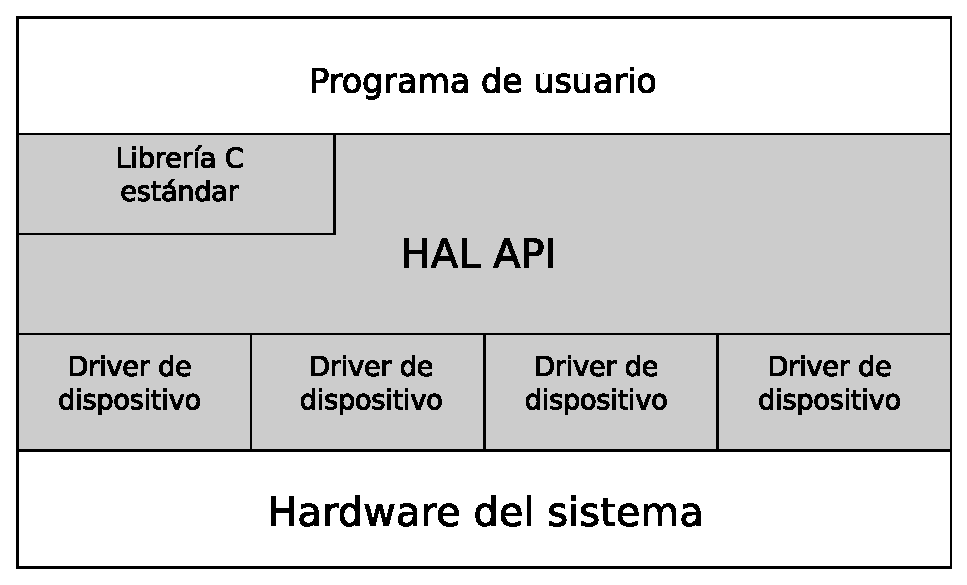
\includegraphics[width=0.80\textwidth]{3-arquitectura/graf/hal.eps}
  \caption{Capas de un sistema basado en la HAL.}
  \label{fig:hal}
\end{figure}

\subsubsection*{Modelos de dispositivos genéricos}

La HAL provee modelos de dispositivos genéricos para diversos tipos de periféricos que se encuentran en sistemas embebidos, tales como timers, interfaces Ethernet y dispositivos de I/O que transmiten datos de caracter. Estos modelos permiten escribir programas usando una API consistente sin preocuparse por el hardware subyacente. Los tipos de periféricos cubiertos son:

\begin{itemize}
	\item Dispositivos de caracter: envían y/o reciben caracteres en forma serial, como ser una UART.
	\item Timers: dispositivos que llevan la cuenta de los tics de un clock y pueden generar interrupciones periódicas.
	\item Subsistemas de archivos: un mecanismo para acceder a archivos almacenados en dispositivos físicos. Dependiendo de la implementación interna, el driver del subsistema de archivos podría acceder a los dispositivos subyacentes en forma directa o usar un driver aparte.
	\item Dispositivos Ethernet: proveen acceso a una conexión Ethernet para un stack de red, tal como la NicheStack® TCP/IP Stack, provista por Altera.
	\item Dispositivos DMA: periféricos que llevan a cabo una gran cantidad de transacciones de datos. El origen y destino pueden ser la propia memoria o algún otro dispositivo.
	\item Dispositivos con memoria flash: periféricos con memoria no volátil que utilizan un protocolo especial de programación para almacenar datos.
\end{itemize}

Todos los periféricos, ya sean de Altera o de terceros, deben proveer un archivo de cabecera que defina la interfaz de bajo nivel del dispositivo con el hardware. 

Ciertos dispositivos tienen características específicas de hardware con requerimientos de uso que no se adaptan bien a una API de propósito general. La HAL maneja dichos requerimientos mediante la función ioctl(), cuyas opciones dependerán del periférico en cuestión.

Algunos periféricos proveen funciones de acceso dedicadas que no están basadas en el modelo genérico de la HAL. En ese caso, se debe proveer un archivo de cabecera con dichas funciones.


\subsubsection*{Librería C estándar : newlib}
La HAL integra su entorno de rutinas con una implementación open-source de la librería C estándar:\textbf{ newlib}. La misma está hecha para ser utilizada en sistemas embebidos. 

\subsubsection*{La HAL dentro de un proyecto de software}
La creación y administración de proyectos basados en la HAL están altamente ligadas al NIOS II SBT. La figura ~\ref{fig:halsof} muestra el diagrama en bloques de un software basado en la HAL. Todo programa de este tipo consta de dos proyectos. El código de aplicación específico se encuentra en uno de ellos, el cual depende a su vez de otro proyecto BSP separado. El primero contiene todo el código que el programador desarrolla. El segundo, toda la información necesaria para la interacción hardware-software. Este último a su vez depende del hardware del sistema, cuya información se encuentra en un archivo generado por la herramienta SOPC Builder.

\begin{figure}[h]
  \centering
	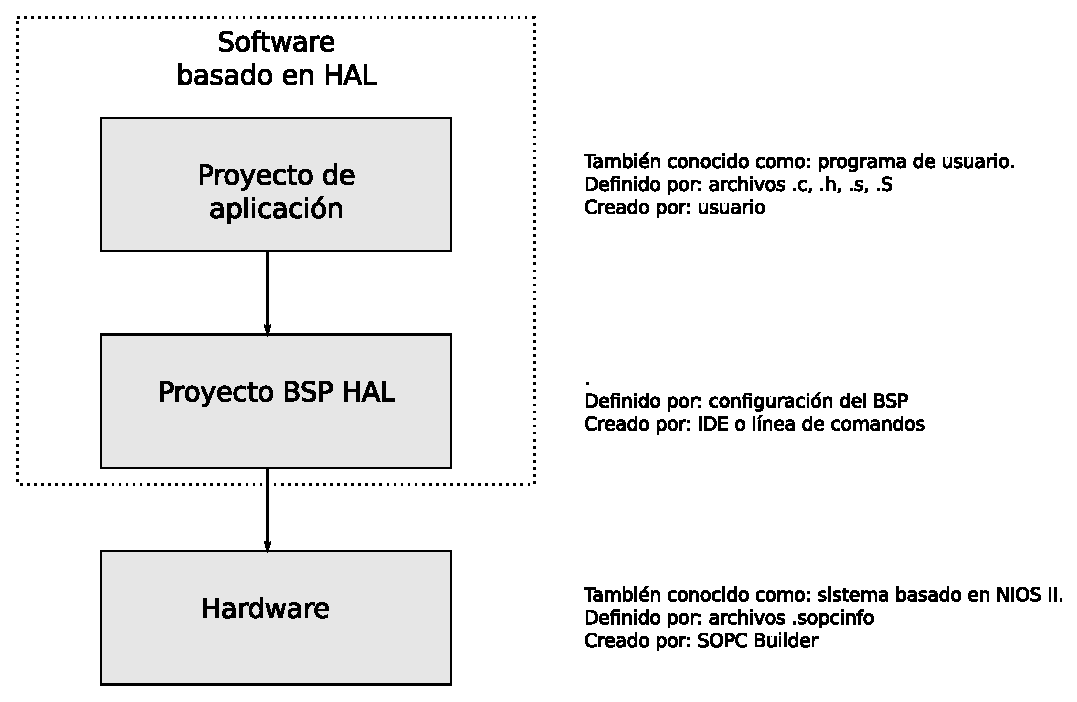
\includegraphics[width=0.90\textwidth]{3-arquitectura/graf/halsof.eps}
  \caption{Capas de un programa basado en HAL}
  \label{fig:halsof}
\end{figure}



\subsubsection*{Archivo de descripción del sistema (system.h)}
El archivo system.h provee una descripción completa del software del sistema basado en NIOS II. Describe cada periférico e incluye:

\begin{itemize}
	\item La configuración de hardware del periférico.
	\item La dirección base.
	\item Información IRQ (si es necesario).
	\item Un nombre simbólico para el periférico.
\end{itemize}

El SBT genera un archivo \textbf{system.h} para cada proyecto BSP, cuyo contenido dependerá del archivo .sopcinfo mencionado anteriormente en este capítulo.

\subsubsection*{Acceso al hardware}
El software accede al hardware a través de macros que abstraen la interfaz mapeada en memoria al dispositivo. Todos los componentes proveen un directorio que define el hardware y el software del periférico en cuestión. En esta carpeta se encuentra un archivo de cabecera que define la interfaz con el hardware y su nombre es $<componente>$\_regs.h, el cual se incluye en el subdirectorio inc. Por ejemplo, el componente JTAG UART define su interfaz en el archivo $<Directorio Instalacion Altera>$/ip/altera/sopc\_builder\_ip/

altera\_avalon\_jtag\_uart/inc/altera\_avalon\_jtag\_uart\_regs.h.

El archivo de cabecera \_regs.h define las siguientes macros de acceso para el componente:
\begin{itemize}
	\item Macros de acceso a registros que proveen operaciones de lectura/escritura. Éstas son:
	\begin{itemize}
		\item IORD\_$<NombreDelComponente>$\_$<NombreDelRegistro>$ ($<DireccionBaseDelComponente>$).
		\item IOWR\_$<NombreDelComponente>$\_$<NombreDelRegistro>$ ($<DireccionBaseDelComponente>$, $<Dato>$).
	\end{itemize}
	\item Macros de direccionamiento de registro, que retornan las direcciones físicas de cada uno de ellos. La dirección devuelta es la dirección base del componente + el valor de desplazamiento de registro especificado. Esta macro tiene el nombre de esta forma:
	\begin{itemize}
		\item IOADDR\_$<NombreDelComponente>$\_$<NombreDelRegistro>$ ($<DireccionBaseDelComponente>$).
	\end{itemize}
	\item Máscaras a nivel de bits. Estas macros tienen los siguientes nombres:
	\begin{itemize}
		\item $<NombreDelComponente>$\_$<NombreDelRegistro>$\_$<NombreDelCampo>$\_MSK : Máscara de bit de un campo.
		\item $<NombreDelComponente>$\_$<NombreDelRegistro>$\_$<NombreDelCampo>$\_OFST : Desplazamiento de bit del el comienzo del campo.
	\end{itemize}
\end{itemize}

Cabe mencionar que las los valores leídos/escritos mediante las macros de acceso a registro (IORD e IOWR) no trabajan con la caché del microprocesador.
En este contexto, es necesario destacar esto ya que los valores intercambiados entre el módulo software y el gestor de datos tienen que ser leidos/escritos solamente si estos están en el bus.

\chapter{Apéndice D}
\section*{SOPC Builder}

SOPC Builder es una herramienta que posibilita la definición y generación de Sistemas en Chips Programables (system-on-a-programable-chip, SOPC) en mucho menos tiempo que requieren los métodos manuales tradicionales de integración. Es parte del software Quartus II.

\subsection*{Componentes a medida (Custom Component)}

Además de una lista de componentes que ya están preparados para funcionar, SOPC Builder ofrece la posibilidad de crear componentes personalizados. Esto se efectúa importando módulos creados en algún HDL.

 Para integrarlos al diseño del sistema se siguen los siguientes pasos:
\begin{enumerate}
	\item Determinar las interfaces necesarias para interactuar con el componente.
	\item Crear la lógica del componente con algún HDL.
	\item Usar el editor de componentes de SOPC Builder para crear el componente a partir de los archivos HDL.
	\item Instanciar el componente en el sistema 
\end{enumerate}

\begin{figure}[H]
  \centering
	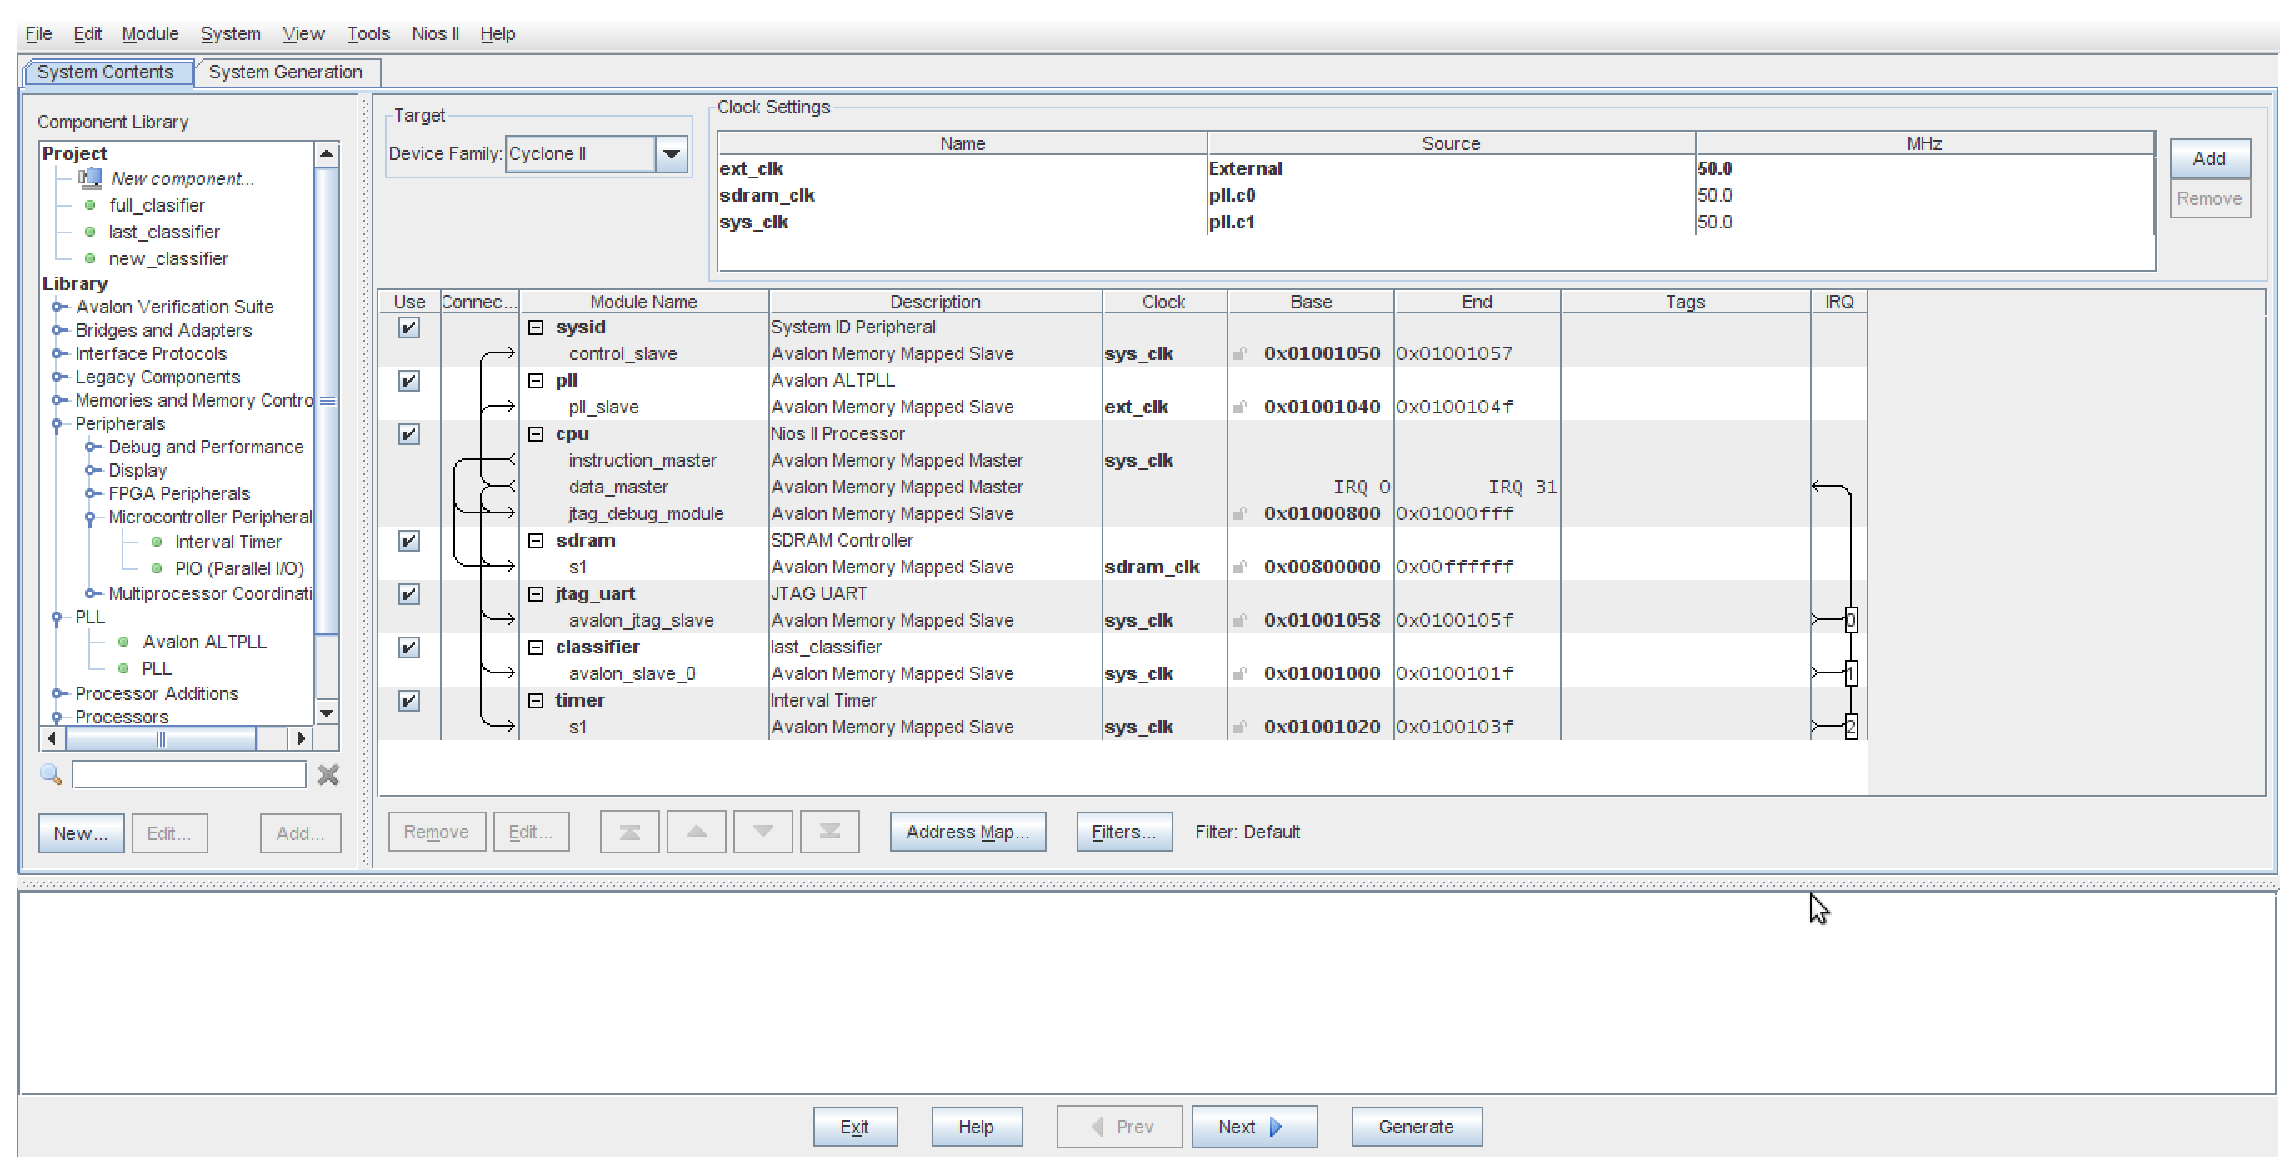
\includegraphics[width=0.90\textwidth]{8-apendices/graf/sopc1.eps}
  \caption{Ventana principal del SOPC Builder}
  \label{fig:sopc1}
\end{figure}

\begin{figure}[H]
  \centering
	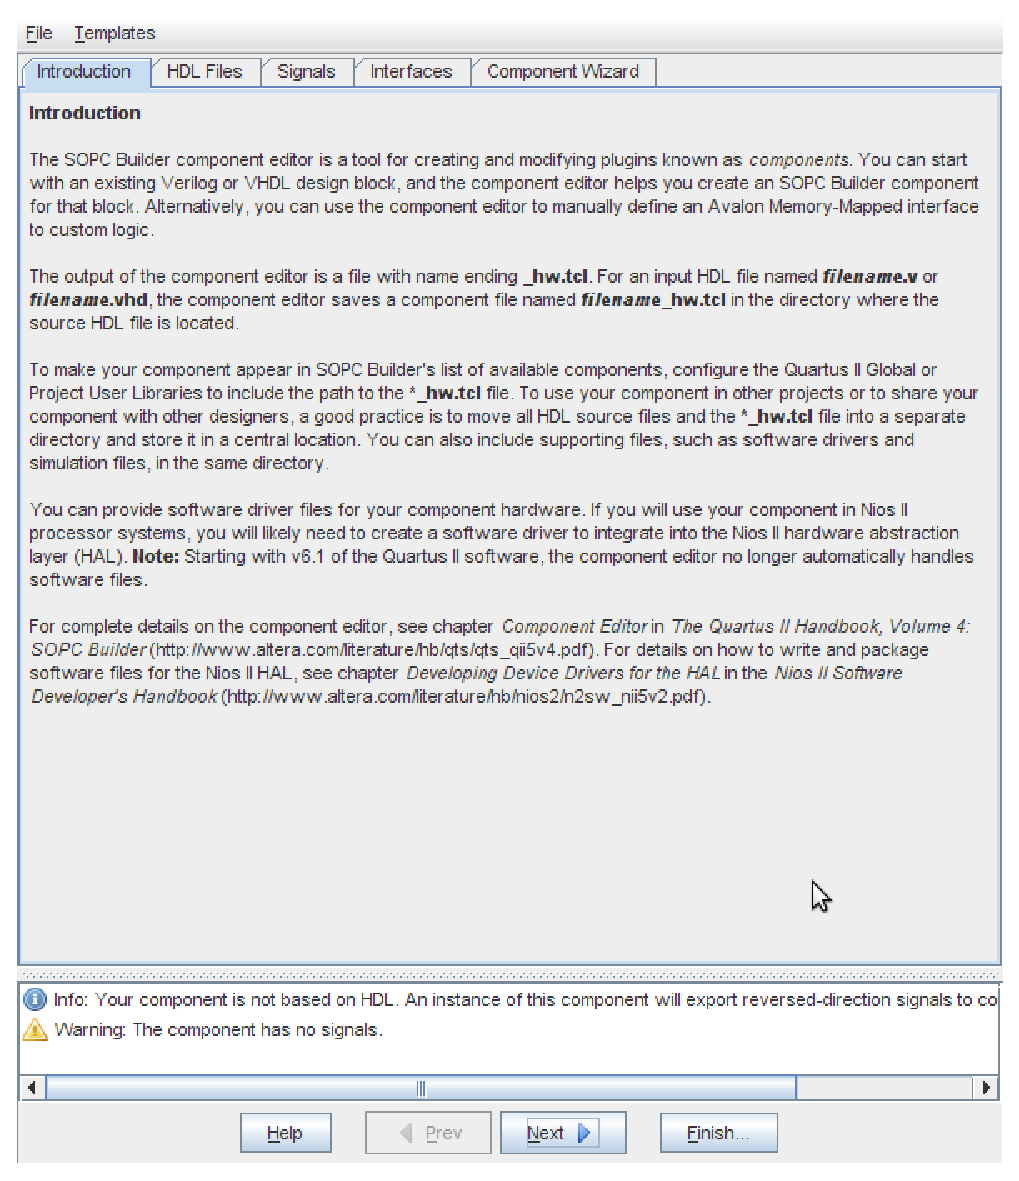
\includegraphics[width=0.60\textwidth]{8-apendices/graf/sopc2.eps}
  \caption{Generador de componentes}
  \label{fig:sopc2}
\end{figure}
